\documentclass[11pt, a4paper]{article}

\usepackage{mlt-thesis-2015}

\usepackage[english]{babel}
\usepackage[hidelinks]{hyperref}
\usepackage{graphicx}
\usepackage{setspace}
\usepackage{comment}
\usepackage{caption}

\usepackage[acronym]{glossaries}
\glsdisablehyper

\title{Visual question answering with type theory}
\subtitle{Using \gls{ttr} to model visual perception and language}
\author{Arild Matsson}
\date{}

\newacronym{hmm}{HMM}{Hidden Markov Model}
\newacronym{lstm}{LSTM}{Long Short-Term Memory}
\newacronym{cnn}{CNN}{convolutional neural network}
\newacronym{ttr}{TTR}{type theory with records}
\newacronym{nlg}{NLG}{natural language generation}
\newacronym{vqa}{VQA}{visual question answering}
\newacronym{yolo}{YOLO}{You only look once}
\newacronym{nlp}{NLP}{natural language processing}

\begin{document}

%% ============================================================================
%% Title page
%% ============================================================================
\begin{titlepage}

\maketitle

\vfill

\begingroup
\renewcommand*{\arraystretch}{1.2}
\begin{tabular}{l@{\hskip 20mm}l}
\hline
Master's Thesis: & 30 credits\\
Programme: & Master’s Programme in Language Technology\\
Level: & Advanced level \\
Semester and year: & Spring, 2018\\
Supervisors & Simon Dobnik and Staffan Larsson\\
Examiner & (name of the examiner)\\
Keywords & type theory, image recognition, object recognition, visual question answering
\end{tabular}
\endgroup

\thispagestyle{empty}
\end{titlepage}

%% ============================================================================
%% Abstract
%% ============================================================================
\newpage
\singlespacing
\section*{Abstract}

%\begin{abstract}
I'm connecting an off-the-shelf image recognition system to PyTTR, a Python implementation of TTR.
This enables representing concepts in the image as TTR types.
Then I'm implementing a \gls{vqa} task.
Questions are represented in TTR through really simple text parsing, and are answered using the representation of the image recognition results.
This shows that \gls{ttr} is helpful for representing visual perception, semantics and cognition.
\glsresetall
%\end{abstract}

\thispagestyle{empty}

%% ============================================================================
%% Preface
%% ============================================================================
\newpage
\section*{Preface}

Acknowledgements, etc.

\thispagestyle{empty}

%% ============================================================================
%% Contents
%% ============================================================================
\newpage

\begin{spacing}{0.0}
\tableofcontents
\end{spacing}

\thispagestyle{empty}

%% ============================================================================
%% Introduction
%% ============================================================================
\newpage
\setcounter{page}{1}

\section{Introduction}
\label{sec:intro}

(Just copied from the thesis proposal for now...)

This project will explore how \gls{ttr} can be used with an image recognition tasks such as question answering.
How can off-the-shelf image recognition software output be expressed in \gls{ttr}, and what can we do with it?

\begin{itemize}
\item Express image classification results in \gls{ttr}
\item Detect and recognize multiple objects in an image, as well as relationships between them
\begin{itemize}
\item Spatial, geometric relationships such as "above" and "to the left of"
\end{itemize}
\item Question anwering: parsing questions or statements into \gls{ttr} and judging their validity in relation to an image
\end{itemize}

\noindent
Development should focus on utilizing and possibly extending PyTTR, a Python implementation of \gls{ttr} \citep{pyttr}. Image recognition and natural language parsing/generation should use existing solutions as far as possible.

\section{Background}

\cite{BlackburnComputationalsemantics2003}:
FOPC for the win. But "other approaches are both possible and interesting".

\subsection{Perceptual semantics}

\cite{LoganComputationalAnalysisApprehension1996}:
Basic–deictic(–intrinsic) relations.
Perceptual–conceptual representation.
"Computational theory of apprehension": spatial indexing -> reference frame -> ... Instead, we move into the conceptual level, both in perception and language, and evaluate validity from there.
(Drawbacks?)
They present "evidence" for their theory, does that evidence contradict the present approach?

\cite{RegierGroundingspatiallanguage2001a}:
AVS
Four models. AVS.
Many experiments.
Spatial term ratings influenced by: proximal \& center-of-mass orientations, grazing line, distance.

\cite{PustejovskyPerceptualsemanticsconstruction1990}?

\subsection{Type theory}

\subsubsection{Type theory, semantics and \gls{nlp}}

\glsreset{ttr}
\subsection{\Gls{ttr}}

\citep{CooperRecordsRecordTypes2005}:
TTR combines lambda calculus, phrase structure grammar, (DRT), (situation semantics) (what are the latter)?

\gls{ttr} is a formal framework for semantics \citep{CooperRecordsRecordTypes2005}.
It has been employed to model natural language in the context of dialogue, situated agents and spoken language.

\subsubsection{Applications of \gls{ttr}}

\cite{DobnikModellinglanguageaction2012} model a robot that would move around and use laser range scanner or similar to collect points in space, group them into objects and detect spatial relations between them.
\Gls{ttr} is used throughout the model, accounting for perception and cognition.

\subsubsection{PyTTR}

\subsection{Visual object recognition}

\begin{figure}[h]
\label{fig:dogbike_annotated}
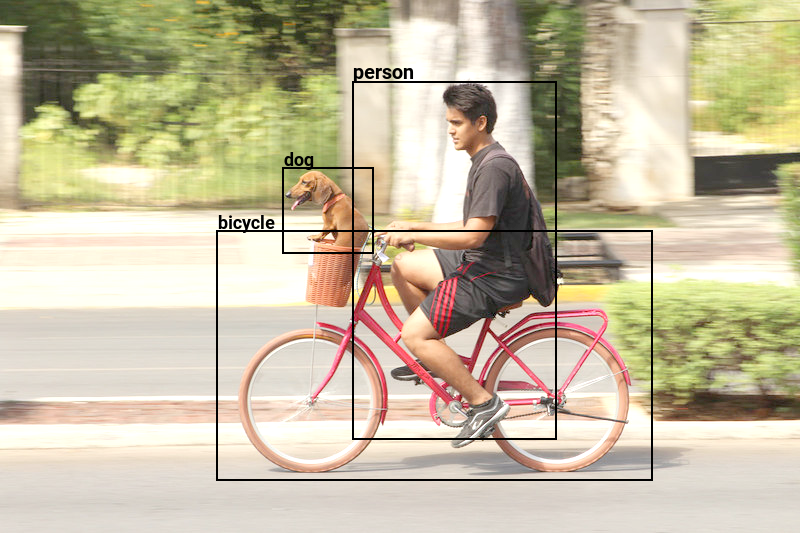
\includegraphics[width=\textwidth]{dogbike_annotated}
\centering
\caption{Visualization of labels and bounding boxes emitted by YOLO given an image depicting a cyclist with a dog.}
\end{figure}

\cite{Detectron2018}

\subsubsection{\Gls{vqa}}

\subsubsection{YOLO object recognition model}

You only look once (YOLO) \citep{RedmonYouOnlyLook2015} is a neural network model that simultaneously predicts bounding boxes around objects and classifies the contained objects.

\section{\Gls{vqa} using \gls{ttr}}

\subsection{Modelling recognised objects}

The off-the-shelf image recognition model is applied to an image.
The output is a set of objects containing bounding box coordinates, a label and a confidence score.
These objects are considered as input to the proposed model.

\begin{equation}\label{eq:seg}
Segment = \left[\begin{array}{rcl}
\text{cy} &:& Int\\
\text{cx} &:& Int\\
\text{w} &:& Int\\
\text{h} &:& Int
\end{array}\right]\end{equation}

\begin{equation}\label{eq:ppty}
Ppty = (Ind\rightarrow Type)\end{equation}

While the confidence score is discarded, the position and the label of each object are used to create a record representing a detected individual.
The type of this record, $Object$, is defined in \autoref{eq:detind} and an example record is given in \autoref{eq:detindrec}.
The $seg$ field is of the type $Segment$, which is defined in \autoref{eq:seg}, and models the position of this object in the image.
The $pfun$ field is of the type $Ppty$, defined in \autoref{eq:ppty} as a function type from $Ind$ to a ptype.
It describes the classification result, a property of the detected object.
The procedure is heavily inspired by Section~5.1 in \cite{DobnikInterfacinglanguagespatial2017}.

\begin{equation}\label{eq:detind}
Object = \left[\begin{array}{rcl}
\text{seg} &:& Segment\\
\text{pfun} &:& Ppty \\
\end{array}\right]\end{equation}

\begin{equation}\label{eq:detindrec}
obj =
\left[\begin{array}{rcl}
\text{seg} &=& \left[\begin{array}{rcl}
\text{cx} &=& 138\\
\text{w} &=& 276\\
\text{cy} &=& 654\\
\text{h} &=& 809
\end{array}\right]\\
\text{pfun} &=& \lambda v:Ind\ .\ \text{person}(v)\\
\end{array}\right] : Object\end{equation}

When the set of detected objects is modeled as a set of $Object$ records, it doesn't say a lot in itself.
What matters is what type they might have.
Types are generated by applying the function $WhatIs$, described in \autoref{eq:whatis}.
The generated types are situations that have been observed.
This is the \textit{basic relation} in \cite{LoganComputationalAnalysisApprehension1996}.


\begin{equation}\label{eq:whatis}
Individualize = \lambda r:Object\ .\ \left[\begin{array}{rcl}
\text{x} &:& Ind\\
\text{loc} &:& Segment_{r.\text{seg}}\\
\text{c}_{prop} &:& r.\text{pfun}(\text{x})\\
\text{c}_{loc} &:& \text{location}(\text{x}, \text{loc})\\
\end{array}\right]\end{equation}

or the "instantiating" version in \autoref{eq:individualizeinst} where $p_i$ are token proofs (?).

\begin{equation}\label{eq:individualizeinst}
Individualize' = \lambda r : Object\ . \left[\begin{array}{lcl}
    \text{x} = a_0 &:& Ind \\
    \text{loc} = r.\text{seg} &:& Segment\\
    \text{cp} = p_0 &:& r.\text{pfun}(\text{x}) \\
    \text{cl} = p_1 &:& \text{location}(\text{x}, \text{loc}) \\
\end{array}\right]
\end{equation}

\begin{equation}\label{eq:ind1}
Individualize(obj) = 
\left[\begin{array}{rcl}
\text{x} &:& Ind\\
\text{loc} &:& Segment_{\left[\begin{array}{rcl}
	\text{cy} &=& 654\\
	\text{h} &=& 809\\
	\text{cx} &=& 138\\
	\text{w} &=& 276
	\end{array}\right]}\\
\text{c}_{prop} &:& \text{person}(\text{x})\\
\text{c}_{loc} &:& \text{location}(\text{x}, \text{loc})\\
\end{array}\right]
\end{equation}

A simple list of the situation types does not provide power enough (??).
They are better combined into one record type that solely describes a situation that includes all the observed situations.

\begin{equation}\label{eq:sitmerge}
\left[\begin{array}{rcl}
\text{x}_\text{8} &:& Ind\\
\text{loc}_\text{8} &:& Segment_{\left[\begin{array}{rcl}
	\text{cy} &=& 191\\
	\text{cx} &=& 508\\
	\text{w} &=& 171\\
	\text{h} &=& 379
	\end{array}\right]}\\
\text{cp}_\text{8} &:& \text{person}(x_{8})\\
\text{cl}_\text{8} &:& \text{location}(x_{8}, loc_{8})\\
\text{x}_\text{9} &:& Ind\\
\text{loc}_\text{9} &:& Segment_{\left[\begin{array}{rcl}
	\text{cy} &=& 288\\
	\text{cx} &=& 496\\
	\text{w} &=& 204\\
	\text{h} &=& 284
	\end{array}\right]}\\
\text{cp}_\text{9} &:& \text{bicycle}(x_{9})\\
\text{cl}_\text{9} &:& \text{location}(x_{9}, loc_{9})\\
\text{x}_\text{10} &:& Ind\\
\text{loc}_\text{10} &:& Segment_{\left[\begin{array}{rcl}
	\text{cy} &=& 384\\
	\text{cx} &=& 210\\
	\text{w} &=& 52\\
	\text{h} &=& 103
	\end{array}\right]}\\
\text{cp}_\text{10} &:& \text{dog}(x_{10})\\
\text{cl}_\text{10} &:& \text{location}(x_{10}, loc_{10})\\
\text{x}_\text{11} &:& Ind\\
\text{loc}_\text{11} &:& Segment_{\left[\begin{array}{rcl}
	\text{cy} &=& 103\\
	\text{cx} &=& 582\\
	\text{w} &=& 90\\
	\text{h} &=& 134
	\end{array}\right]}\\
\text{cp}_\text{11} &:& \text{backpack}(x_{11})\\
\text{cl}_\text{11} &:& \text{location}(x_{11}, loc_{11})\\
\end{array}\right]\end{equation}

\subsection{Spatial relationships}

[spatial relationship classifiers?]

From the information modeled above, how can we see what relationships occur between individuals?

We step back from the merged list-like rectype, to the proper list of $IndObj$ rectypes.
For every pair of such objects, and for every spatial relationship classifier, the pair is evaluated by the classifier.
\autoref{eq:leftclfdef} defines how a classifier $\kappa_{left}$ determines whether the $\text{left}$ relation holds between two objects.

\begin{multline}\label{eq:leftclfdef}
SpatRelClf(pred, \kappa) = 
\lambda r :
\left[\begin{array}{rcl}
    \text{trg}&:&\left[\begin{array}{rcl}
        \text{x}&:&Ind\\
        \text{loc}&:&Segment\\
        \text{cl}&:& \text{location}(\text{x},\text{loc})
    \end{array}\right]\\
    \text{ref}&:&\left[\begin{array}{rcl}
        \text{x}&:&Ind\\
        \text{loc}&:&Segment\\
        \text{cl}&:& \text{location}(\text{x},\text{loc})
    \end{array}\right]\\
\end{array}\right] .\\
\begin{cases}
\left[\begin{array}{lcl}
    \text{trg}=r.\text{trg}.\text{x} &:& Ind\\
    \text{ref}=r.\text{ref}.\text{x} &:& Ind\\
    \text{cr} &:& pred(\text{trg}, \text{ref})\\
\end{array}\right]
& \text{if } \kappa(r.\text{trg}.\text{loc}, r.\text{ref}.\text{loc}) \\
[] & \text{otherwise}
\end{cases}
\end{multline}

This is then added to the list in \autoref{eq:sitmerge}, where $\text{trg}$ and $\text{ref}$ should be eliminated as duplicates, and only $\text{cr}$ remains to be added.
The result is illustrated in \ref{eq:sitmergerels}.
If the classifier $\kappa_{left}$ returns false, of course nothing is to be added.
Negations in TTR are treated by \cite{CooperNegationdialogue2018} but are not considered presently.

\begin{equation}\label{eq:sitmergerels}
\left[\begin{array}{rcl}
\text{x}_\text{9} &:& Ind\\
\text{cp}_\text{9} &:& \text{bicycle}(x_{9})\\
\text{cl}_\text{9} &:& \text{location}(x_{9}, loc_{9})\\
\text{loc}_\text{9} &:& Segment_{\left[\begin{array}{rcl}
	\text{cy} &=& 288\\
	\text{cx} &=& 496\\
	\text{w} &=& 204\\
	\text{h} &=& 284
	\end{array}\right]}\\
\text{x}_\text{10} &:& Ind\\
\text{cp}_\text{10} &:& \text{dog}(x_{10})\\
\text{cl}_\text{10} &:& \text{location}(x_{10}, loc_{10})\\
\text{loc}_\text{10} &:& Segment_{\left[\begin{array}{rcl}
	\text{cy} &=& 384\\
	\text{cx} &=& 210\\
	\text{w} &=& 52\\
	\text{h} &=& 103
	\end{array}\right]}\\
\text{cr}_\text{11} &:& \text{left}(\text{x}_{10}, \text{x}_9)\\
\end{array}\right]\end{equation}


\subsection{Natural language parsing}

A dog is to the left of a car
\begin{equation}\left[\begin{array}{rcl}
\text{x} &:& Ind\\
\text{y} &:& Ind\\
\text{c}_\text{dog} &:& \text{dog}(x)\\
\text{c}_\text{car} &:& \text{car}(y)\\
\text{c}_\text{left} &:& \text{left}(x, y)\\
\end{array}\right]\end{equation}

\subsubsection{Implementation}

NLTK FCFG.
FOPC to RecType.

\subsubsection{Limitations}

Disjunction ("or").


\subsection{Evaluating propositions (answering questions)}

Essentially, we would like to check if the situation observed is a subtype of the situation described by the text/question, whether $Q \sqsupseteq A$. A new problem here is that field labels do not match, even if the field values (the types) match. We thus need to consider all (?) relabelings of $Q$:

A record type $T_1$ is a \textbf{relabel-subtype} of $T_2$ if there is a relabeling of $T_1$, $T_{1_{rlb}}$ where $T_{1_{rlb}} \sqsubseteq T_2$.

Could we forget field labels and just look at the two sets of field values? Not really, because we have dependent types, so $\text{dog}(x_1) ≠ \text{dog}(x_2)$. We need to carry out each candidate \textit{relabeling} and check subtypeness. In practice, and in this case, relabeling the basic-type ($Ind$) fields is enough, because those are the only ones whose labels appear in dependent fields. For each basic-field relabeling, we can then kind of forget labels and just find subtypeness of field values.

[Relabel-subtype pseudocode]

\section{Conclusions}

\subsection{Future work}

Basic->Deictic->Intrinsic relations  \cite{LoganComputationalAnalysisApprehension1996}

Spatial templates \& regions of acceptability. Compound relations (above right) finer (directly). Functional aspect.  \cite{LoganComputationalAnalysisApprehension1996} (also Dobnik etc)

4 question types.

Classification after Q.

Probabilistic TTR for "good fit" (is is more to the left or more above?).

Moar question types (tasks/programs/routines in L\&S).

\bibliography{imagettr}
\end{document}